% Options for packages loaded elsewhere
\PassOptionsToPackage{unicode}{hyperref}
\PassOptionsToPackage{hyphens}{url}
%
\documentclass[
]{article}

\usepackage[a4paper,top=2cm,bottom=1.5cm,left=2cm,right=2cm,marginparwidth=1.5cm]{geometry}
\usepackage[utf8]{inputenc}
\usepackage{textcomp}
\usepackage{graphicx}
\usepackage{lmodern}
\usepackage{amssymb,amsmath}
\usepackage{ifxetex,ifluatex}
\usepackage{bm}
\usepackage[french]{babel}
\usepackage[T1]{fontenc}
\usepackage[myheadings]{fullpage}
\DeclareUnicodeCharacter{0301}{\hspace{-1ex}\'{ }}
\usepackage{fancyhdr}
\usepackage{lastpage}

% For figures and stuff
\usepackage{graphicx, wrapfig, subcaption, setspace, booktabs}
\usepackage[T1]{fontenc}

% Change for different font sizes and families
\usepackage[font=small, labelfont=bf]{caption}
\usepackage{fourier}
% Maths
\usepackage{tabto}
\usepackage{amsmath,amssymb}
\usepackage{float}
\usepackage{graphicx}
\usepackage{wrapfig}
\usepackage[colorinlistoftodos]{todonotes}
\usepackage[colorlinks=true, allcolors=blue]{hyperref}
\usepackage{listings}
\usepackage{lmodern}
\usepackage{amssymb,amsmath}
\usepackage{ifxetex,ifluatex}

\ifnum 0\ifxetex 1\fi\ifluatex 1\fi=0 % if pdftex
\usepackage[T1]{fontenc}
  \usepackage[utf8]{inputenc}
  \usepackage{textcomp} % provide euro and other symbols
  \else % if luatex or xetex
  \usepackage{unicode-math}
  \defaultfontfeatures{Scale=MatchLowercase}
  \defaultfontfeatures[\rmfamily]{Ligatures=TeX,Scale=1}
  \fi
  % Use upquote if available, for straight quotes in verbatim environments
  \IfFileExists{upquote.sty}{\usepackage{upquote}}{}
  \IfFileExists{microtype.sty}{% use microtype if available
\usepackage[]{microtype}
\UseMicrotypeSet[protrusion]{basicmath} % disable protrusion for tt fonts
}{}
\makeatletter
\@ifundefined{KOMAClassName}{% if non-KOMA class
\IfFileExists{parskip.sty}{%
\usepackage{parskip}
}{% else
\setlength{\parindent}{0pt}
    \setlength{\parskip}{6pt plus 2pt minus 1pt}}
    }{% if KOMA class
  \KOMAoptions{parskip=half}}
  \makeatother
  \usepackage{xcolor}
\IfFileExists{xurl.sty}{\usepackage{xurl}}{} % add URL line breaks if available
\IfFileExists{bookmark.sty}{\usepackage{bookmark}}{\usepackage{hyperref}}
\hypersetup{
  hidelinks,
  pdfcreator={LaTeX via pandoc}}
\urlstyle{same} % disable monospaced font for URLs
\usepackage{color}
% Use upquote if available, for straight quotes in verbatim environments
\IfFileExists{upquote.sty}{\usepackage{upquote}}{}
\IfFileExists{microtype.sty}{% use microtype if available
  \usepackage[]{microtype}
  \UseMicrotypeSet[protrusion]{basicmath} % disable protrusion for tt fonts
}{}
\makeatletter
\@ifundefined{KOMAClassName}{% if non-KOMA class
  \IfFileExists{parskip.sty}{%
    \usepackage{parskip}
  }{% else
    \setlength{\parindent}{0pt}
    \setlength{\parskip}{6pt plus 2pt minus 1pt}}
}{% if KOMA class
  \KOMAoptions{parskip=half}}
\makeatother
\usepackage{xcolor}
\IfFileExists{xurl.sty}{\usepackage{xurl}}{} % add URL line breaks if available
\IfFileExists{bookmark.sty}{\usepackage{bookmark}}{\usepackage{hyperref}}
\hypersetup{
  pdftitle={Systeme Expert pour l'aide à la réalisation de prêts bancaires},
  hidelinks,
  pdfcreator={LaTeX via pandoc}}
\urlstyle{same} % disable monospaced font for URLs
\usepackage{color}
\usepackage{fancyvrb}
\newcommand{\VerbBar}{|}
\newcommand{\VERB}{\Verb[commandchars=\\\{\}]}
\DefineVerbatimEnvironment{Highlighting}{Verbatim}{commandchars=\\\{\}}
% Add ',fontsize=\small' for more characters per line
\newenvironment{Shaded}{}{}
\newcommand{\AlertTok}[1]{\textcolor[rgb]{1.00,0.00,0.00}{\textbf{#1}}}
\newcommand{\AnnotationTok}[1]{\textcolor[rgb]{0.38,0.63,0.69}{\textbf{\textit{#1}}}}
\newcommand{\AttributeTok}[1]{\textcolor[rgb]{0.49,0.56,0.16}{#1}}
\newcommand{\BaseNTok}[1]{\textcolor[rgb]{0.25,0.63,0.44}{#1}}
\newcommand{\BuiltInTok}[1]{#1}
\newcommand{\CharTok}[1]{\textcolor[rgb]{0.25,0.44,0.63}{#1}}
\newcommand{\CommentTok}[1]{\textcolor[rgb]{0.38,0.63,0.69}{\textit{#1}}}
\newcommand{\CommentVarTok}[1]{\textcolor[rgb]{0.38,0.63,0.69}{\textbf{\textit{#1}}}}
\newcommand{\ConstantTok}[1]{\textcolor[rgb]{0.53,0.00,0.00}{#1}}
\newcommand{\ControlFlowTok}[1]{\textcolor[rgb]{0.00,0.44,0.13}{\textbf{#1}}}
\newcommand{\DataTypeTok}[1]{\textcolor[rgb]{0.56,0.13,0.00}{#1}}
\newcommand{\DecValTok}[1]{\textcolor[rgb]{0.25,0.63,0.44}{#1}}
\newcommand{\DocumentationTok}[1]{\textcolor[rgb]{0.73,0.13,0.13}{\textit{#1}}}
\newcommand{\ErrorTok}[1]{\textcolor[rgb]{1.00,0.00,0.00}{\textbf{#1}}}
\newcommand{\ExtensionTok}[1]{#1}
\newcommand{\FloatTok}[1]{\textcolor[rgb]{0.25,0.63,0.44}{#1}}
\newcommand{\FunctionTok}[1]{\textcolor[rgb]{0.02,0.16,0.49}{#1}}
\newcommand{\ImportTok}[1]{#1}
\newcommand{\InformationTok}[1]{\textcolor[rgb]{0.38,0.63,0.69}{\textbf{\textit{#1}}}}
\newcommand{\KeywordTok}[1]{\textcolor[rgb]{0.00,0.44,0.13}{\textbf{#1}}}
\newcommand{\NormalTok}[1]{#1}
\newcommand{\OperatorTok}[1]{\textcolor[rgb]{0.40,0.40,0.40}{#1}}
\newcommand{\OtherTok}[1]{\textcolor[rgb]{0.00,0.44,0.13}{#1}}
\newcommand{\PreprocessorTok}[1]{\textcolor[rgb]{0.74,0.48,0.00}{#1}}
\newcommand{\RegionMarkerTok}[1]{#1}
\newcommand{\SpecialCharTok}[1]{\textcolor[rgb]{0.25,0.44,0.63}{#1}}
\newcommand{\SpecialStringTok}[1]{\textcolor[rgb]{0.73,0.40,0.53}{#1}}
\newcommand{\StringTok}[1]{\textcolor[rgb]{0.25,0.44,0.63}{#1}}
\newcommand{\VariableTok}[1]{\textcolor[rgb]{0.10,0.09,0.49}{#1}}
\newcommand{\VerbatimStringTok}[1]{\textcolor[rgb]{0.25,0.44,0.63}{#1}}
\newcommand{\WarningTok}[1]{\textcolor[rgb]{0.38,0.63,0.69}{\textbf{\textit{#1}}}}
\usepackage{graphicx}
\makeatletter
\def\maxwidth{\ifdim\Gin@nat@width>\linewidth\linewidth\else\Gin@nat@width\fi}
\def\maxheight{\ifdim\Gin@nat@height>\textheight\textheight\else\Gin@nat@height\fi}
\makeatother
% Scale images if necessary, so that they will not overflow the page
% margins by default, and it is still possible to overwrite the defaults
% using explicit options in \includegraphics[width, height, ...]{}


\setkeys{Gin}{width=\maxwidth,height=\maxheight,keepaspectratio}

% Set default figure placement to htbp
\makeatletter
\def\fps@figure{htbp}
\makeatother
\setlength{\emergencystretch}{3em} % prevent overfull lines
\providecommand{\tightlist}{%
  \setlength{\itemsep}{0pt}\setlength{\parskip}{0pt}}
\setcounter{secnumdepth}{-\maxdimen} % remove section numbering

\usepackage{fancyhdr}
\usepackage{incgraph}
\usepackage{qtree}
\usepackage{algorithm}
\usepackage{pdfpages}
\usepackage{amsmath}
\usepackage{amssymb}

\newcommand{\HRule}[1]{\rule{\linewidth}{#1}}
\onehalfspacing
\setcounter{tocdepth}{5}
\setcounter{secnumdepth}{5}


\pagestyle{fancy}
% \pagestyle{fancy}
\fancyhf{}

% Header and footer information
\setlength\headheight{15pt}

\fancyfoot[R]{\thepage}
 \setlength{\marginparwidth}{2cm}
\usepackage[
    left = \flqq{},% 
    right = \frqq{},% 
    leftsub = \flq{},% 
    rightsub = \frq{} %
    ]{dirtytalk}
    \pagestyle{fancy}
    \setlength\headheight{15pt}
    \fancyhead[L]{SAVARY Tobias BAUVAIS Camille UTC - GI01} 
    \fancyhead[R]{IA01 - Rapport TP3}
    \fancyfoot[R]{\thepage}
    \fancyfoot[L]{Université de Technologie de Compiègne}
     \setlength {\marginparwidth}{2cm}
     \renewcommand{\footrulewidth}{.5pt}
     
     
     

\begin{document}

\title{Rapport de stage}
\author{Tobias SAVARY}
\date{}

\title{ \begin{center}
          
\includegraphics[width=5cm]{img/logo_IA01.png} \hspace*{1cm}
          
\includegraphics[width=9cm]{img/logo_UTC.png} \\ [2cm]
  \end{center}
  % Change to your faculty if needed
		\HRule{2pt} \\
		\LARGE \textbf{Rapport TP3:\\Système Expert \\ Aide à la réalisation de prêts bancaires} 
		\HRule{2pt} \\ [5.5cm]
		\normalsize  
        \author{
            Tobias SAVARY \\[0.5cm]
            Camille BAUVAIS \\[1cm]
      \today
        }
		}
        
		\maketitle
        \begin{center}
            Année universitaire 2022/2023
        \end{center}
\pagebreak

\tableofcontents
\pagebreak

\hypertarget{introduction}{%
\section{Introduction}\label{introduction}}

Lors de ce TP3, nous avons réalisé le développement d'un système-expert
d'ordre 0+ de sa phase d'expertise à sa phase d'utilisation. Pour cela,
nous avons tout d'abord réfléchi à différents sujets possibles. Nous
avions plusieurs idées telles que : des systèmes d'aides à la décision
pour le choix d'une voiture en fonction du profil du client et de ses
besoins, un outil d'aide à la réalisation de prêts bancaires, un outil
pour accorder son vin avec son plat, un outil pour le choix des UVs ou
encore la reconnaissance de plante en fonctions de leurs
caractéristiques. Suite à plusieurs réflexions et mises en commun, nous
avons décidé de choisir l'aide à la réalisation de prêts bancaires. En
effet, ce sujet nous semblait le plus approprié et intéressant car il
constitue un sujet concret. De plus, en tant qu'étudiant, on peut avoir
à réaliser un prêt étudiant, et dans notre vie future nous seront
sûrement amenés à faire des prêts pour l'achat d'une voiture ou d'une
maison par exemple. Lors d'un prêt étudiant, ce qui nous intéresse est
le montant que l'on aura à rembourser par mois une fois que l'on sera
diplômé, une partie de notre futur salaire sera dédiée au remboursement
du prêt et il est important de savoir à quelle hauteur il s'élèvera.\\
Il est souvent compliqué de savoir si l'on est éligible à tel ou tel
prêt. Ou encore de savoir si nos revenus sont suffisants pour supporter
le remboursement d'un prêt sur le long terme.\\
L'interface finale de notre projet a pour objectif de clarifier ce type
de questions. Elle est dédiée à tout particulier souhaitant réaliser un
prêt, pas seulement pour le personnel bancaire.

Ce choix nous permettait aussi d'appliquer des chaînages avant et
arrière vus dans le cadre de ce cours.

L'objectif de notre système-expert est de répondre à 3 problématiques
majeures :\\
1. Un prêt est-il faisable ?\\
2. Quel sera le montant à rembourser chaque mois ?\\
3. Quelle sera la durée du prêt ?

Pour répondre à la première question, nous allons demander à
l'utilisateur toutes les informations nécessaires et effectuer des
chaînages avant et arrière pour voir si un prêt est envisageable selon
les critères précédemment renseignés.\\
Pour les deux autres questions, nous effectuons un chainage avant
puis nous réalisons le calcul demandé (durée ou montant).

Afin de mener à bien ce projet, nous nous sommes documentés sur les
différentes possibilités de prêts et leurs conditions respectives.\\
Cette recherche documentaire nous a permis de déterminer les
connaissances nécessaires au système-expert et de créer notre base de
règle associée.

\pagebreak

\hypertarget{explication-de-la-base-de-ruxe8gles}{%
\section{Explication de la base de
règles}\label{explication-de-la-base-de-ruxe8gles}}

Durant ce projet, nous avons décidé de traiter trois prêts majeurs, qui
sont :\\
\tabto{1cm} - le prêt immobilier\\
\tabto{1cm} - le prêt étudiant\\
\tabto{1cm} - le crédit à la consommation

La source experte provient de nombreux sites internet, que ce soit des
banques ou des simulateurs préexistants. Les différents sites consultés
sont référencés dans les sources.\\
A partir de cette source d'expertise, nous avons pu créer notre base de
règles. La bdr regroupe, pour chaque type de prêt, les caractéristiques
permettant sa réalisation ainsi que tous les attributs qui le concerne
:\\
\tabto{1cm} - taux\\
\tabto{1cm} - montant min\\
\tabto{1cm} - montant max\\
\tabto{1cm} - durée min\\
\tabto{1cm} - durée max\\
\tabto{1cm} - endettement\\
\tabto{1cm} - critèreApport\\
\tabto{1cm} - profession\\
\tabto{1cm} - ...

Explication des termes utilisés : \\
\tabto{0.5cm} - Endettement qui représente le taux d'endettement. Ce taux détermine le montant qu'un emprunteur peut
raisonnablement consacrer au remboursement d'un crédit tout en
continuant à vivre correctement. On le calcule de la manière suivante :
endettement= $(mensualités ×100)/(revenus mensuels)$ \\ \\
\tabto{0.5cm} - Critère apport qui est un indicateur sur l'apport fournit par l'utilisateur. On considère
que l'apport est suffisamment important lorsqu'il permet de couvrir les
frais de dossier, soit environ 10\% du montant du prêt. Ainsi ce critère
est placé à 1 s'il représente au moins 10\% du montant et à 0 sinon.

Au final pour avoir un prêt immobilier accepté il faut que la personne
soit de nationalité française ou ait vécu en France depuis au moins 5
ans, qu'elle ait une situation stable c'est-à-dire un CDI, être
fonctionnaire ou avoir des revenus suffisamment élevés, que son taux
d'endettement soit inférieur à 35\%, que son critère de l'apport soit
supérieur ou égal à 1, que la durée de son prêt soit comprise entre 7 et
25 ans et que le montant soit supérieur à 50000€.

Pour que le prêt soit refusé, il faut que la personne soit âgée de plus
de 65 et qu'elle n'ait souscrit à aucune assurance.

Pour les prêts à la consommation on demande le type parmi travaux, auto
et personnel car les taux changent en fonction du type sélectionné.

\pagebreak
\hypertarget{base-de-ruxe8gles}{%
\subsection{Base de règles}\label{base-de-ruxe8gles}}

Voici la base de règles que nous avons mise en place pour la réalisation de ce projet :

\begin{Shaded}
\begin{Highlighting}[]
\NormalTok{(}\KeywordTok{setq}\NormalTok{ *bdr*}
\NormalTok{\textquotesingle{}(( R1 ((}\KeywordTok{eq}\NormalTok{ profession CDI)) (}\KeywordTok{eq}\NormalTok{ situation stable))}
\NormalTok{( R2 ((}\KeywordTok{eq}\NormalTok{ profession fonctionnaire)) (}\KeywordTok{eq}\NormalTok{ situation stable))}
\NormalTok{( R3 ((}\OperatorTok{\textgreater{}=}\NormalTok{ revenu }\DecValTok{5000}\NormalTok{)) (}\KeywordTok{eq}\NormalTok{ situation stable))}
\NormalTok{( R4 ((}\KeywordTok{eq}\NormalTok{ nationalite France)(}\OperatorTok{\textgreater{}=}\NormalTok{ age }\DecValTok{18}\NormalTok{)) (}\KeywordTok{eq}\NormalTok{ statut Francais))}
\NormalTok{( R5 ((}\KeywordTok{eq}\NormalTok{ lieuResidence France) (}\OperatorTok{\textgreater{}=}\NormalTok{ duree\_sejour }\DecValTok{5}\NormalTok{) (}\OperatorTok{\textgreater{}=}\NormalTok{ age }\DecValTok{18}\NormalTok{)) (}\KeywordTok{eq}\NormalTok{ statut Francais))}
\NormalTok{( R6 ((}\KeywordTok{eq}\NormalTok{ profession etudiant) (}\KeywordTok{eq}\NormalTok{ statut Francais) (}\OperatorTok{\textless{}=}\NormalTok{ age }\DecValTok{28}\NormalTok{)) (}\KeywordTok{eq}\NormalTok{ StatutEtu valide))}
\NormalTok{( R7 ((}\OperatorTok{\textgreater{}}\NormalTok{ age }\DecValTok{65}\NormalTok{) (}\OperatorTok{\textgreater{}}\NormalTok{ duree\_pret }\DecValTok{7}\NormalTok{)) (}\KeywordTok{eq}\NormalTok{ etatPret refuse))}
\NormalTok{( R8 ((}\OperatorTok{\textgreater{}}\NormalTok{ age }\DecValTok{65}\NormalTok{) (}\KeywordTok{eq}\NormalTok{ assurance non)) (}\KeywordTok{eq}\NormalTok{ etatPret refuse))}
\NormalTok{( R9 ((}\KeywordTok{eq}\NormalTok{ situation stable)(}\OperatorTok{\textless{}}\NormalTok{ endettement }\DecValTok{35}\NormalTok{)) (}\KeywordTok{eq}\NormalTok{ typePret credit))}
\NormalTok{( R10 ((}\OperatorTok{\textgreater{}=}\NormalTok{ critereApport }\DecValTok{1}\NormalTok{) (}\KeywordTok{eq}\NormalTok{ typePret credit) (}\KeywordTok{eq}\NormalTok{ statut Francais)) }
\NormalTok{        (}\KeywordTok{eq}\NormalTok{ typePret Immobilier) )}
\NormalTok{( R11 ((}\KeywordTok{eq}\NormalTok{ typePret Immobilier)(}\OperatorTok{\textless{}=}\NormalTok{ duree\_pret }\DecValTok{27}\NormalTok{) (}\OperatorTok{\textgreater{}=}\NormalTok{ duree\_pret }\DecValTok{5}\NormalTok{) (}\OperatorTok{\textgreater{}=}\NormalTok{ montant }\DecValTok{50000}\NormalTok{)) }
\NormalTok{        (}\KeywordTok{eq}\NormalTok{ etatPret accepte))}
\NormalTok{( R12 ((}\KeywordTok{eq}\NormalTok{ typePret Immobilier)) (}\OperatorTok{\textgreater{}=}\NormalTok{ montant }\DecValTok{50000}\NormalTok{))}
\NormalTok{( R13 ((}\KeywordTok{eq}\NormalTok{ typePret Immobilier)) (}\OperatorTok{\textless{}=}\NormalTok{ duree\_pret }\DecValTok{27}\NormalTok{))}
\NormalTok{( R14 ((}\KeywordTok{eq}\NormalTok{ typePret Immobilier)) (}\OperatorTok{\textgreater{}=}\NormalTok{ duree\_pret }\DecValTok{5}\NormalTok{))}
\NormalTok{( R15 ((}\KeywordTok{eq}\NormalTok{ typePret Immobilier) (}\OperatorTok{\textless{}=}\NormalTok{ duree\_pret }\DecValTok{10}\NormalTok{)) (}\OperatorTok{=}\NormalTok{ taux }\FloatTok{2.40}\NormalTok{))}
\NormalTok{( R16 ((}\KeywordTok{eq}\NormalTok{ typePret Immobilier) (}\OperatorTok{\textless{}=}\NormalTok{ duree\_pret }\DecValTok{15}\NormalTok{)(}\OperatorTok{\textgreater{}}\NormalTok{ duree\_pret }\DecValTok{10}\NormalTok{)) (}\OperatorTok{=}\NormalTok{ taux }\FloatTok{2.53}\NormalTok{))}
\NormalTok{( R17 ((}\KeywordTok{eq}\NormalTok{ typePret Immobilier) (}\OperatorTok{\textless{}=}\NormalTok{ duree\_pret }\DecValTok{20}\NormalTok{)(}\OperatorTok{\textgreater{}}\NormalTok{ duree\_pret }\DecValTok{15}\NormalTok{)) (}\OperatorTok{=}\NormalTok{ taux }\FloatTok{2.64}\NormalTok{))}
\NormalTok{( R18 ((}\KeywordTok{eq}\NormalTok{ typePret Immobilier) (}\OperatorTok{\textgreater{}=}\NormalTok{ duree\_pret }\DecValTok{20}\NormalTok{)) (}\OperatorTok{=}\NormalTok{ taux }\FloatTok{2.81}\NormalTok{))}
\NormalTok{( R19 ((}\KeywordTok{eq}\NormalTok{ statutEtu valide)) (}\KeywordTok{eq}\NormalTok{ typePret Etudiant))}
\NormalTok{( R20 ((}\KeywordTok{eq}\NormalTok{ typePret Etudiant) (}\OperatorTok{\textgreater{}=}\NormalTok{ montant }\DecValTok{1500}\NormalTok{) (}\OperatorTok{\textless{}=}\NormalTok{ montant }\DecValTok{30000}\NormalTok{) }
\NormalTok{(}\OperatorTok{\textgreater{}=}\NormalTok{ duree\_pret }\DecValTok{2}\NormalTok{) (}\OperatorTok{\textless{}=}\NormalTok{ duree\_pret }\DecValTok{10}\NormalTok{)) (}\KeywordTok{eq}\NormalTok{ etatPret accepte))}
\NormalTok{( R21 ((}\KeywordTok{eq}\NormalTok{ typePret Etudiant)) (}\OperatorTok{\textless{}=}\NormalTok{ montant }\DecValTok{30000}\NormalTok{))}
\NormalTok{( R22 ((}\KeywordTok{eq}\NormalTok{ typePret Etudiant)) (}\OperatorTok{\textgreater{}=}\NormalTok{ montant }\DecValTok{1500}\NormalTok{))}
\NormalTok{( R23 ((}\KeywordTok{eq}\NormalTok{ typePret Etudiant)) (}\OperatorTok{=}\NormalTok{ taux }\FloatTok{2.00}\NormalTok{))}
\NormalTok{( R24 ((}\KeywordTok{eq}\NormalTok{ typePret Etudiant)) (}\OperatorTok{\textless{}=}\NormalTok{ duree\_pret }\DecValTok{10}\NormalTok{))}
\NormalTok{( R25 ((}\KeywordTok{eq}\NormalTok{ typePret Etudiant)) (}\OperatorTok{\textgreater{}=}\NormalTok{ duree\_pret }\DecValTok{2}\NormalTok{))}

\NormalTok{( R26 ((}\KeywordTok{eq}\NormalTok{ typePret credit)(}\KeywordTok{eq}\NormalTok{ statut Francais)) (}\KeywordTok{eq}\NormalTok{ typePret consommation))}
\NormalTok{( R27 ((}\KeywordTok{eq}\NormalTok{ typePret consommation)(}\OperatorTok{\textless{}}\NormalTok{ montant }\DecValTok{50000}\NormalTok{)(}\OperatorTok{\textgreater{}=}\NormalTok{ duree\_pret }\DecValTok{1}\NormalTok{)(}\OperatorTok{\textless{}=}\NormalTok{ duree\_pret }\DecValTok{6}\NormalTok{)) }
\NormalTok{        (}\KeywordTok{eq}\NormalTok{ etatPret accepte))}
\NormalTok{( R28 ((}\KeywordTok{eq}\NormalTok{ typePret consommation)) (}\OperatorTok{\textless{}=}\NormalTok{ duree\_pret }\DecValTok{6}\NormalTok{))}
\NormalTok{( R29 ((}\KeywordTok{eq}\NormalTok{ typePret consommation)) (}\OperatorTok{\textgreater{}=}\NormalTok{ duree\_pret }\DecValTok{1}\NormalTok{))}
\NormalTok{( R30 ((}\KeywordTok{eq}\NormalTok{ typePret consommation)) (}\OperatorTok{\textless{}}\NormalTok{ montant }\DecValTok{50000}\NormalTok{))}

\NormalTok{( R31 ((}\KeywordTok{eq}\NormalTok{ typePret consommation)(}\KeywordTok{eq}\NormalTok{ typeConso auto)(}\OperatorTok{=}\NormalTok{ duree\_pret }\DecValTok{1}\NormalTok{)) }
\NormalTok{    (}\OperatorTok{=}\NormalTok{ taux }\FloatTok{0.51}\NormalTok{))}
\NormalTok{( R32 ((}\KeywordTok{eq}\NormalTok{ typePret consommation)(}\KeywordTok{eq}\NormalTok{ typeConso auto)(}\OperatorTok{\textless{}=}\NormalTok{ duree\_pret }\DecValTok{2}\NormalTok{)(}\OperatorTok{\textgreater{}}\NormalTok{ duree\_pret }\DecValTok{1}\NormalTok{)) }
\NormalTok{    (}\OperatorTok{=}\NormalTok{ taux }\FloatTok{1.51}\NormalTok{))}
\NormalTok{( R33 ((}\KeywordTok{eq}\NormalTok{ typePret consommation)(}\KeywordTok{eq}\NormalTok{ typeConso auto)(}\OperatorTok{\textless{}=}\NormalTok{ duree\_pret }\DecValTok{3}\NormalTok{)(}\OperatorTok{\textgreater{}}\NormalTok{ duree\_pret }\DecValTok{2}\NormalTok{)) }
\NormalTok{    (}\OperatorTok{=}\NormalTok{ taux }\FloatTok{1.91}\NormalTok{))}
\NormalTok{( R34 ((}\KeywordTok{eq}\NormalTok{ typePret consommation)(}\KeywordTok{eq}\NormalTok{ typeConso auto)(}\OperatorTok{\textless{}=}\NormalTok{ duree\_pret }\DecValTok{5}\NormalTok{)(}\OperatorTok{\textgreater{}}\NormalTok{ duree\_pret }\DecValTok{3}\NormalTok{)) }
\NormalTok{    (}\OperatorTok{=}\NormalTok{ taux }\FloatTok{2.41}\NormalTok{))}
\NormalTok{( R35 ((}\KeywordTok{eq}\NormalTok{ typePret consommation)(}\KeywordTok{eq}\NormalTok{ typeConso auto)(}\OperatorTok{\textless{}=}\NormalTok{ duree\_pret }\DecValTok{6}\NormalTok{)(}\OperatorTok{\textgreater{}}\NormalTok{ duree\_pret }\DecValTok{5}\NormalTok{)) }
\NormalTok{    (}\OperatorTok{=}\NormalTok{ taux }\FloatTok{3.41}\NormalTok{))}

\NormalTok{( R36 ((}\KeywordTok{eq}\NormalTok{ typePret consommation)(}\KeywordTok{eq}\NormalTok{ typeConso travaux)(}\OperatorTok{=}\NormalTok{ duree\_pret }\DecValTok{1}\NormalTok{)) (}\OperatorTok{=}\NormalTok{ taux }\FloatTok{0.91}\NormalTok{))}
\NormalTok{( R37 ((}\KeywordTok{eq}\NormalTok{ typePret consommation)(}\KeywordTok{eq}\NormalTok{ typeConso travaux)(}\OperatorTok{\textless{}=}\NormalTok{ duree\_pret }\DecValTok{2}\NormalTok{)(}\OperatorTok{\textgreater{}}\NormalTok{ duree\_pret }\DecValTok{1}\NormalTok{)) }
\NormalTok{    (}\OperatorTok{=}\NormalTok{ taux }\FloatTok{2.01}\NormalTok{))}
\NormalTok{( R38 ((}\KeywordTok{eq}\NormalTok{ typePret consommation)(}\KeywordTok{eq}\NormalTok{ typeConso travaux)(}\OperatorTok{\textless{}=}\NormalTok{ duree\_pret }\DecValTok{3}\NormalTok{)(}\OperatorTok{\textgreater{}}\NormalTok{ duree\_pret }\DecValTok{2}\NormalTok{)) }
\NormalTok{    (}\OperatorTok{=}\NormalTok{ taux }\FloatTok{2.41}\NormalTok{))}
\NormalTok{( R39 ((}\KeywordTok{eq}\NormalTok{ typePret consommation)(}\KeywordTok{eq}\NormalTok{ typeConso travaux)(}\OperatorTok{\textless{}=}\NormalTok{ duree\_pret }\DecValTok{4}\NormalTok{)(}\OperatorTok{\textgreater{}}\NormalTok{ duree\_pret }\DecValTok{3}\NormalTok{)) }
\NormalTok{    (}\OperatorTok{=}\NormalTok{ taux }\FloatTok{2.80}\NormalTok{))}
\NormalTok{( R40 ((}\KeywordTok{eq}\NormalTok{ typePret consommation)(}\KeywordTok{eq}\NormalTok{ typeConso travaux)(}\OperatorTok{\textless{}=}\NormalTok{ duree\_pret }\DecValTok{5}\NormalTok{)(}\OperatorTok{\textgreater{}}\NormalTok{ duree\_pret }\DecValTok{4}\NormalTok{)) }
\NormalTok{    (}\OperatorTok{=}\NormalTok{ taux }\FloatTok{3.00}\NormalTok{))}
\NormalTok{( R41 ((}\KeywordTok{eq}\NormalTok{ typePret consommation)(}\KeywordTok{eq}\NormalTok{ typeConso travaux)(}\OperatorTok{\textless{}=}\NormalTok{ duree\_pret }\DecValTok{6}\NormalTok{)(}\OperatorTok{\textgreater{}}\NormalTok{ duree\_pret }\DecValTok{5}\NormalTok{)) }
\NormalTok{    (}\OperatorTok{=}\NormalTok{ taux }\FloatTok{3.40}\NormalTok{))}

\NormalTok{( R42 ((}\KeywordTok{eq}\NormalTok{ typePret consommation)(}\KeywordTok{eq}\NormalTok{ typeConso personnel)(}\OperatorTok{=}\NormalTok{ duree\_pret }\DecValTok{1}\NormalTok{)) (}\OperatorTok{=}\NormalTok{ taux }\FloatTok{0.51}\NormalTok{))}
\NormalTok{( R43 ((}\KeywordTok{eq}\NormalTok{ typePret consommation)(}\KeywordTok{eq}\NormalTok{ typeConso personnel)(}\OperatorTok{\textless{}=}\NormalTok{ duree\_pret }\DecValTok{2}\NormalTok{)(}\OperatorTok{\textgreater{}}\NormalTok{ duree\_pret }\DecValTok{1}\NormalTok{)) }
\NormalTok{    (}\OperatorTok{=}\NormalTok{ taux }\FloatTok{1.51}\NormalTok{))}
\NormalTok{( R44 ((}\KeywordTok{eq}\NormalTok{ typePret consommation)(}\KeywordTok{eq}\NormalTok{ typeConso personnel)(}\OperatorTok{\textless{}=}\NormalTok{ duree\_pret }\DecValTok{3}\NormalTok{)(}\OperatorTok{\textgreater{}}\NormalTok{ duree\_pret }\DecValTok{2}\NormalTok{)) }
\NormalTok{    (}\OperatorTok{=}\NormalTok{ taux }\FloatTok{1.91}\NormalTok{))}
\NormalTok{( R45 ((}\KeywordTok{eq}\NormalTok{ typePret consommation)(}\KeywordTok{eq}\NormalTok{ typeConso personnel)(}\OperatorTok{\textless{}=}\NormalTok{ duree\_pret }\DecValTok{4}\NormalTok{)(}\OperatorTok{\textgreater{}}\NormalTok{ duree\_pret }\DecValTok{3}\NormalTok{)) }
\NormalTok{    (}\OperatorTok{=}\NormalTok{ taux }\FloatTok{2.80}\NormalTok{))}
\NormalTok{( R46 ((}\KeywordTok{eq}\NormalTok{ typePret consommation)(}\KeywordTok{eq}\NormalTok{ typeConso personnel)(}\OperatorTok{\textless{}=}\NormalTok{ duree\_pret }\DecValTok{5}\NormalTok{)(}\OperatorTok{\textgreater{}}\NormalTok{ duree\_pret }\DecValTok{4}\NormalTok{)) }
\NormalTok{    (}\OperatorTok{=}\NormalTok{ taux }\FloatTok{2.41}\NormalTok{))}
\NormalTok{( R47 ((}\KeywordTok{eq}\NormalTok{ typePret consommation)(}\KeywordTok{eq}\NormalTok{ typeConso personnel)(}\OperatorTok{\textless{}=}\NormalTok{ duree\_pret }\DecValTok{6}\NormalTok{)(}\OperatorTok{\textgreater{}}\NormalTok{ duree\_pret }\DecValTok{5}\NormalTok{)) }
\NormalTok{    (}\OperatorTok{=}\NormalTok{ taux }\FloatTok{4.51}\NormalTok{))}
\NormalTok{))}
\end{Highlighting}
\end{Shaded}

\hypertarget{arbre-de-duxe9duction}{%
\subsection{Arbre de déduction}\label{arbre-de-duxe9duction}}

Voici l'arbre de déduction correspondant à la base de règles ci-dessus :

Le premier arbre permet de représenter toutes les règles jusqu'à R25 et
le second permet de représenter les règles suivantes (elles sont
principalement liées au prêt à la consommation).

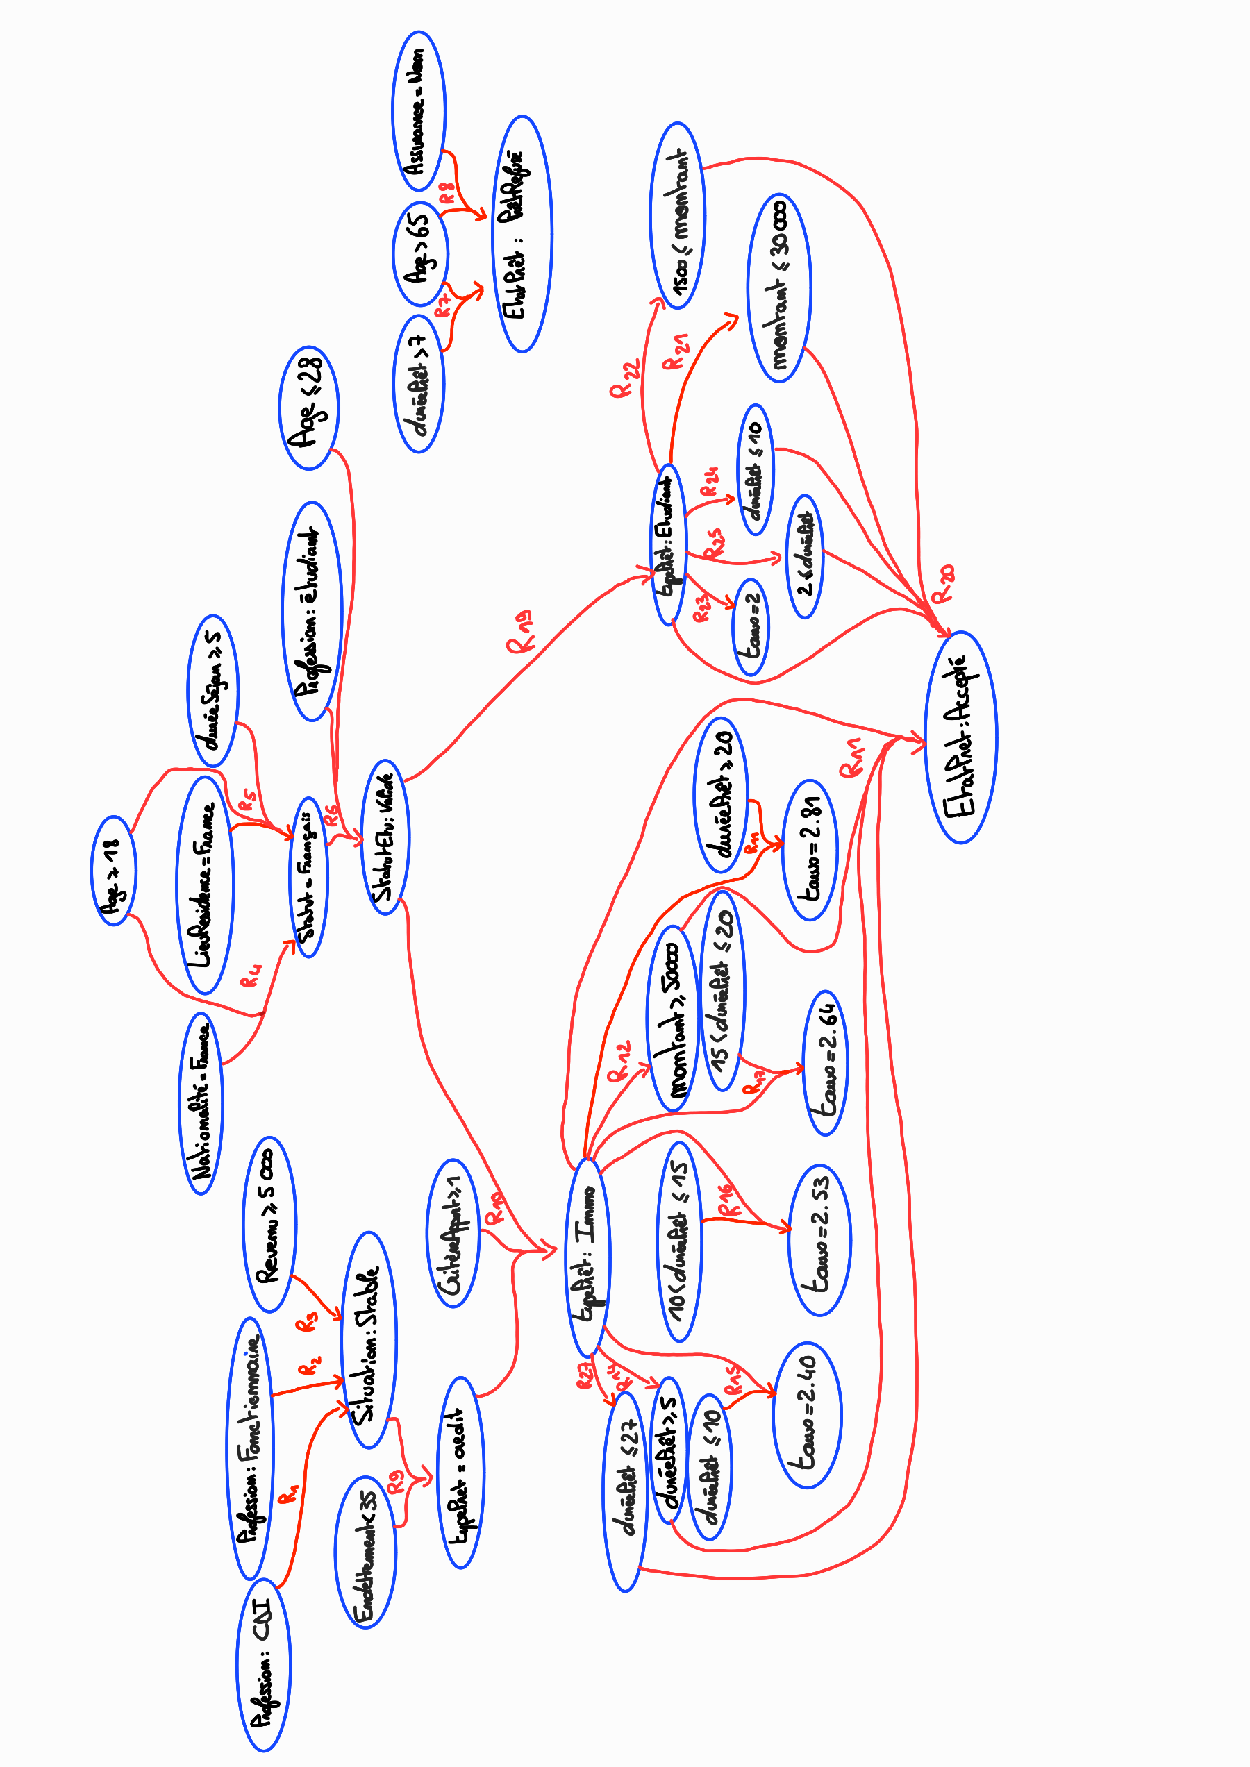
\includepdf[width=17cm, page=1]{img/Arbre_TP3.pdf}
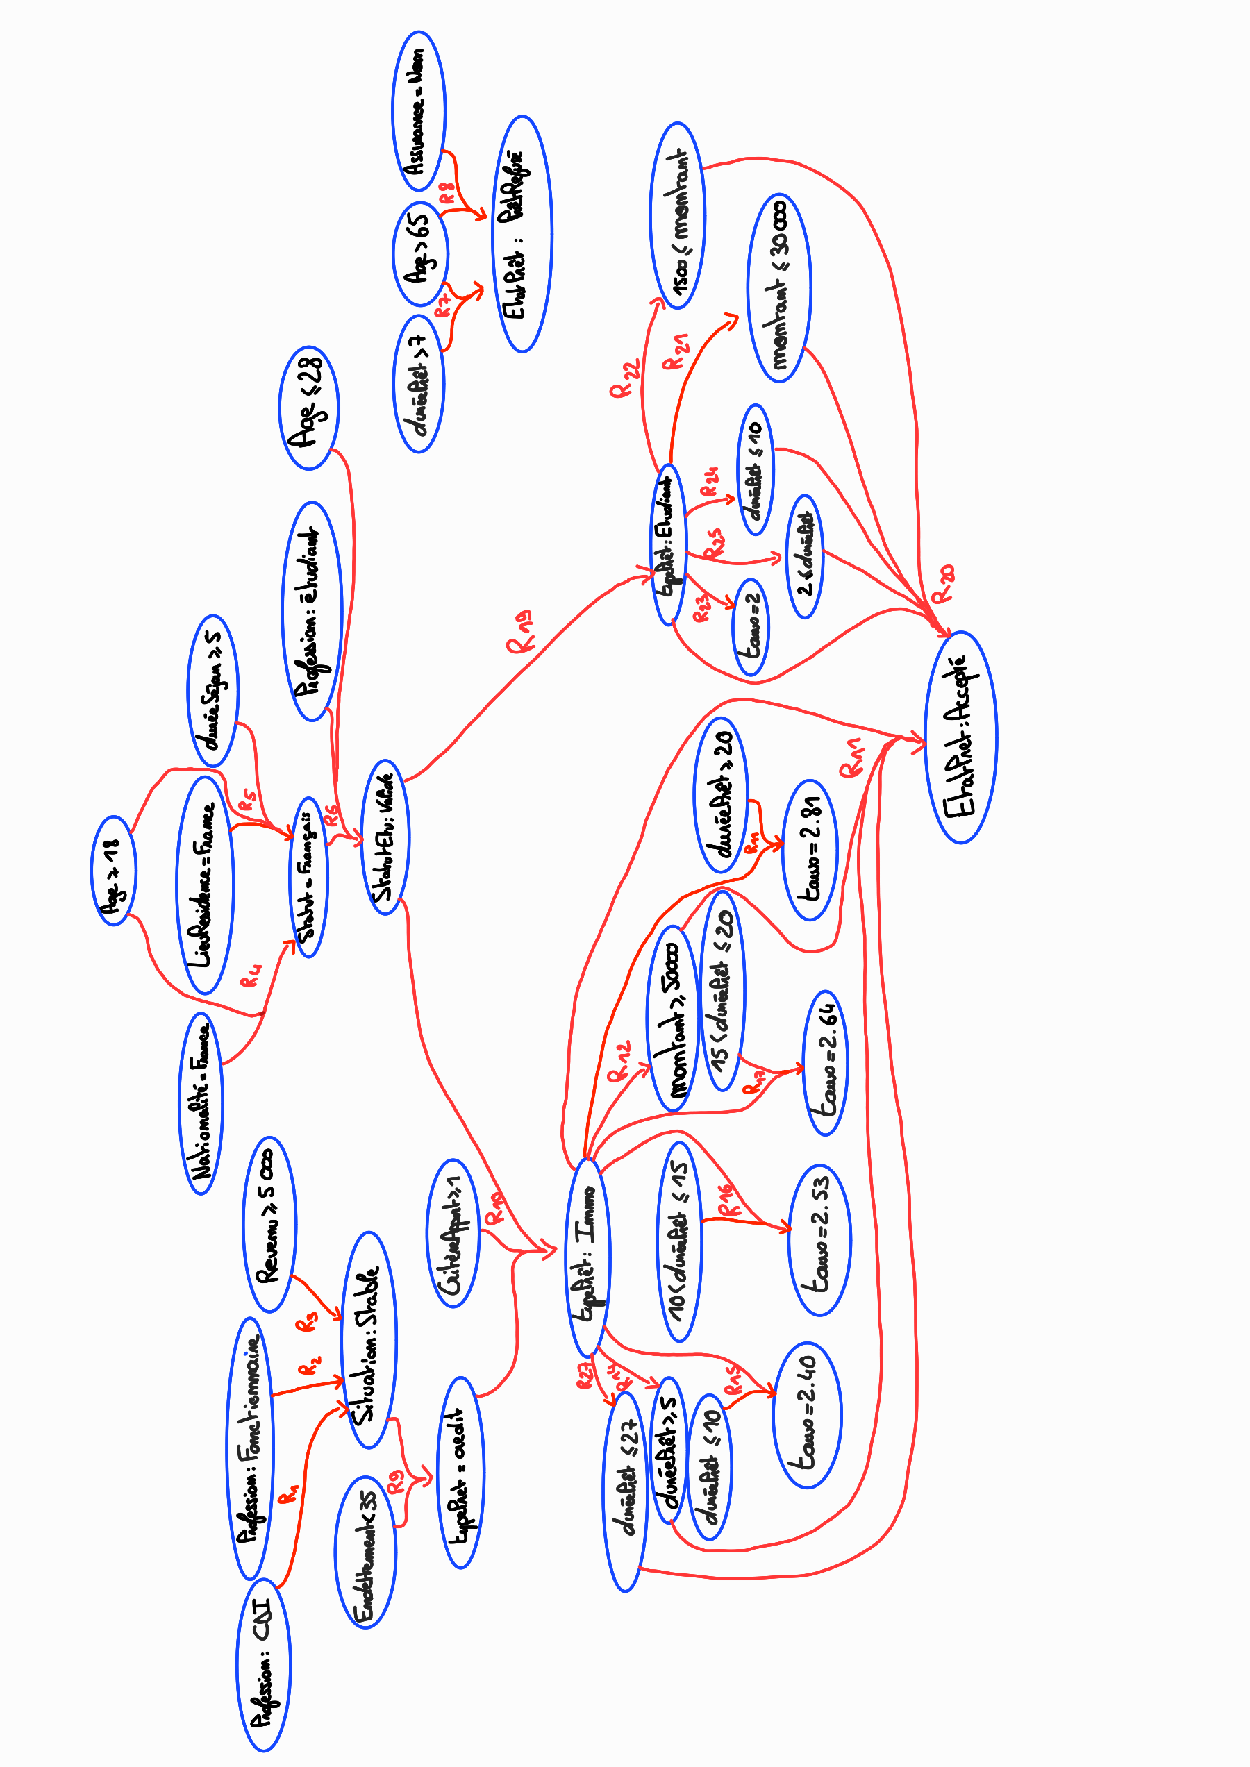
\includepdf[width=17cm, page=2]{img/Arbre_TP3.pdf}

\hypertarget{sources}{%
\subsection{Sources}\label{sources}}

Les sources suivantes nous ont permis d'élaborer notre base de règles :

Pour le \textbf{prêt immobilier} : \\
\begin{itemize}
\item
\url{https://edito.seloger.com/conseils-d-experts/acheter/les-conditions-d-obtention-d-un-pret-immobilier-book.html} \\
\item
\url{https://www.pretto.fr/pret-immobilier/conditions-credit-immobilier/} \\
\item
\url{https://www.pretto.fr/pret-immobilier/conseils/duree-pret-immobilier/} \\
\end{itemize}
Pour le \textbf{prêt étudiant} : \\
\begin{itemize}
\item
\url{https://www.banquepopulaire.fr/conseils/conditions-pret-etudiant/} \\
\end{itemize}
Pour le \textbf{crédit à la consommation} : \\
\begin{itemize}
\item
\url{https://www.nos-economies.fr/credit-consommation/conditions-obtention-credit-conso/} \\
\item
\url{https://www.nos-economies.fr/credit-consommation/comparateur-credit-conso/} \\
\item
\url{https://www.credit-agricole.fr} \\
\end{itemize}

\pagebreak

\hypertarget{impluxe9mentation}{%
\section{Implémentation}\label{impluxe9mentation}}

\hypertarget{explication-des-moteurs-dinfuxe9rence-choisis}{%
\subsection{Explication des moteurs d'inférence
choisis}\label{explication-des-moteurs-dinfuxe9rence-choisis}}

Avec cette bdr nous avons décidé de réaliser un menu proposant 3 choix
afin de répondre aux trois problématiques mentionnées dans
l'introduction. 

Le premier étant pour tester la faisabilité du prêt :\\
Dans la fonction fpret, on réalise un chaînage arrière afin de savoir si
les informations rentrées par l'utilisateur permettent d'arriver à la
conclusion (eq etatPret accepte). Ce chaînage arrière s'effectue en
profondeur sur la bdr puisqu'il parcourt les règles comportant la
conclusion (eq typePret credit) (eq situation stable) (eq typePret
`immobilier ou `etudiant ou `consommation) et (eq statut français).
Avant de réaliser ce chaînage arrière, on effectue un autre chaînage
arrière sur la conclusion (eq etatPret refuse) pour vérifier si
l'utilisateur n'a pas entré d'informations qui pouvaient compromettre
son prêt, notamment un âge avancé. \\
A la fin de la fonction, si le chainage\_arrière n'a pas aboutit à la 
réalisation du prêt, nous envoyons un message indiquant qu'elle critère
empêche la réalisation du prêt. Cela est plus détaillé un peu plus bas, 
au moment de l'explication du chainage arrière. \\ \\
Ensuite, le menu propose le calcul de la mensualité :\\
La fonction calculmensualité permet, pour un type de prêt donné et une
durée, de récupérer à l'aide d'un chaînage avant le taux correspondant
afin de calculer le montant que l'emprunteur aura à rembourser chaque
mois. A noter que cette fonction est utilisée dans la première partie du
menu également. Ce calcul s'effectue de la manière suivante :
\begin{equation}
\frac{montant * (1+ \frac{taux}{100})}{durée * 12} \\
\end{equation}

Enfin, la troisième proposition permet de
fournir une durée pour le remboursement d'un prêt :\\
La fonction duree\_remboursement calcule la durée nécessaire de
remboursement d'un prêt à l'aide d'un montant et d'un critère de
mensualité donné. Ce critère de mensualité définit le montant que
l'emprunteur souhaite rembourser par mois. \\

Remarque : pour pouvoir connaitre le taux à appliquer nous avons 
besoin de la durée du prêt, or dans ce cas elle nous 
est inconnue. Le chainage avant pour trouver le taux 
selon le type de prêt nous renvoie le taux le plus 
élevé (cela s'explique par le fait que la base de fait 
s'enrichit du maximum de la durée possible en tant que 
durée\_pret). Alors, suite au calcul, on obtient une 
durée ne correspondant pas parfaitement au taux choisi. 
Pour palier à cette différence, nous réeffectuons un 
chainage avant mais cette fois ci en entrant dans la 
base de fait la durée de prêt qui vient d'être trouvée, 
le taux retourné se rapproche alors davantage de la 
réalité. Ainsi, suite à un deuxième calcul, on retrouve 
une deuxième durée (sensiblement identique si le montant 
n'est pas très élevé) qu'on renvoie. Suite à ce 
deuxième calcul, il se pourrait que le deuxième taux 
ne corresponde toujours pas à la durée trouvée, 
cependant nous avons décidé de ne pas continuer 
cette boucle car nous considérons que le résultat 
changerait extrêment peu par la suite (les taux sont 
généralement autour de 2\% et on remarque de faible 
variations). 

\pagebreak

D'autres fonctions annexes sont employées dans ces fonctions.

On retrouve notamment les getters qui permettent de demander à
l'utilisateur les informations nécessaires afin de remplir la base de
fait à l'aide d'un read pour chaque type de donnée voulue.

Les checkers vérifient à l'aide d'un chaînage avant si le montant
(respectivement la durée) correspond bien au minimum et au maximum de
chaque type de prêt.

Le chaînage arrière est réalisé grâce à la combinaison de la fonction
verfier\_ou et vérifier\_et. Verifier\_ou permet de vérifier si la bdf
permet de vérifier au moins une règle comportant le but voulu. Elle fait
appel (à chaque « ou ») à vérifier\_et qui vérifie pour chaque règle si
la bdf vérifie toutes les prémisses de la règle.\\
Pour des fins d'explicabilité, nous avons modifié la fonction
vérifier\_et et ajouté une variable globale dernier\_enr qui nous permet
d'enregistrer la règle qui n'a pas abouti au succès du chaînage avant.
De ce fait, dans la fonction fpret, un affichage permet d'indiquer
pourquoi le prêt n'est pas faisable. Cela permet d'informer
l'utilisateur, qui sait alors quel critère ne correspond pas afin de
pouvoir le modifier si possible.

Le chaînage avant parcourt toute la bdr, si une règle se vérifie avec la
bdf grâce à la fonction verif\_regle alors quand le premier parcours de
la bdr sera fini, il faudra recommencer puisque la bdf sera enrichie.
Lorsqu'une conclusion comportant le terme recherché est atteinte, on
ajoute la conclusion à une liste résultat qui sera renvoyée à la fin de
l'exécution de la fonction.\\
Lors de l'enrichissement de la bdf, on vérifie que la 
caractéristique n'y est pas déjà présente. Pour les 
conclusions qui contiennent des >= ou <= nous avons 
décidé de les traiter comme s'il s'agissait d'un = puisque 
cela n'affecte pas nos traitements par la suite. \\

Par exemple, si on veut récupérer la durée min et max d'un prêt étudiant.
Il faut effectuer un chainage avant sur duree\_pret, avec une bdf semblable 
à ((type\_pret etudiant)).
La liste résultat contiendra : ((\textgreater= duree\_pret 2)(\textless=
duree\_pret 10)). Ainsi, il ne reste plus qu'à vérifier si la durée
entrée par l'utilisateur est comprise entre ces deux durées, c'est
notamment sur ce principe que fonctionnent les checkers.

\hypertarget{explication-des-ruxe9sultats-obtenus}{%
\subsection{Explication des résultats
obtenus}\label{explication-des-ruxe9sultats-obtenus}}

Pour le bon fonctionnement de notre système-expert, nous avons tout
d'abord mis en place un menu afin de faciliter l'utilisation. 
Ce menu est contenu dans la fonction (menubanque), qu'il
faut appeler pour commencer la simulation. Cette fonction boucle tant 
que l'utilisateur ne demande pas de sortir (choix n°4). Dans un premier
temps, elle propose 4 choix, correspondant à nos trois problématiques + 
la sortie, ensuite elle nous propose de choisir entre les trois types de prêt. 
Une fois tous les choix enregistrés, elle appelle la fonction appropriée 
parmi fpret (faisabilité), calculmensualité (calcul de la mensualité), 
duree\_remboursement (durée du remboursement).

\begin{figure}[H]
\centering
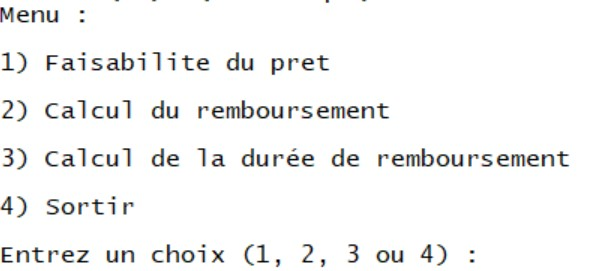
\includegraphics{img/menu.jpg}
\caption{Menu}
\end{figure}

La première fonctionnalité permet de tester la faisabilité d'un prêt.

\begin{figure}[H]
\centering
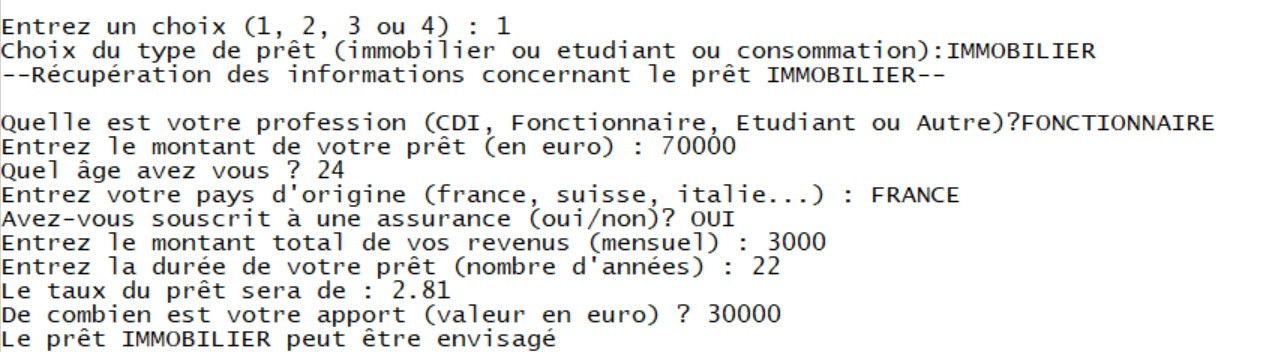
\includegraphics{img/fpret_possible_immo.jpg}
\caption{Faisabilitée d'un prêt immobilier}
\end{figure}

\begin{figure}[H]
\centering
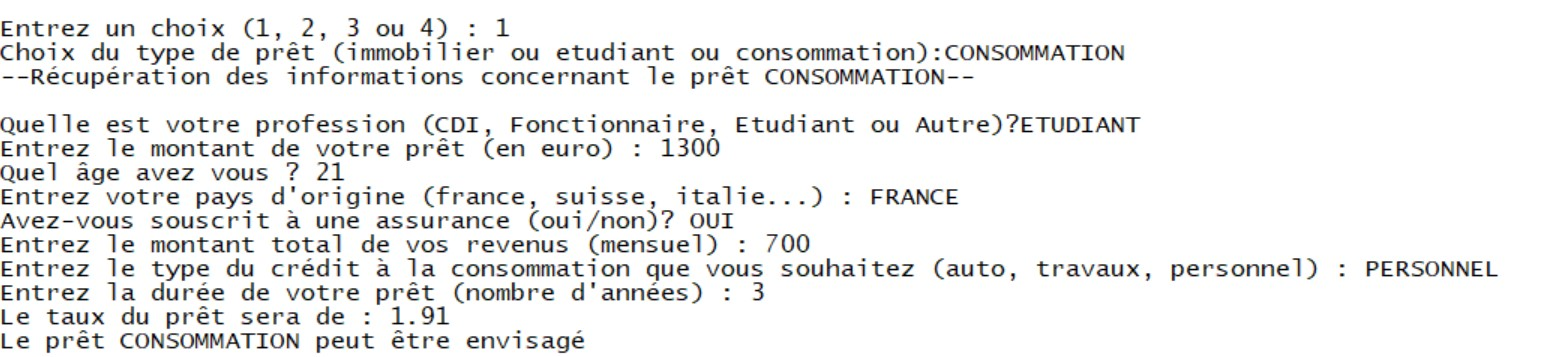
\includegraphics{img/fpret_possible_conso.jpg}
\caption{Faisabilitée d'un prêt à la consommation}
\end{figure}

Dans ces deux exemples, on remarque qu'il est demandé à l'utilisateur
toutes les informations nécessaires au remplissage de la base de fait
qui servira par la suite pour le traitement des informations dans la
fonction fpret. On remarque que dans ces deux exemples les prêts peuvent
être envisageables, car les critères entrés sont corrects et
correspondent à la base de règles.

\pagebreak

Nous avons ensuite deux exemples pour lesquels le prêt est impossible :

\begin{figure}[H]
\centering
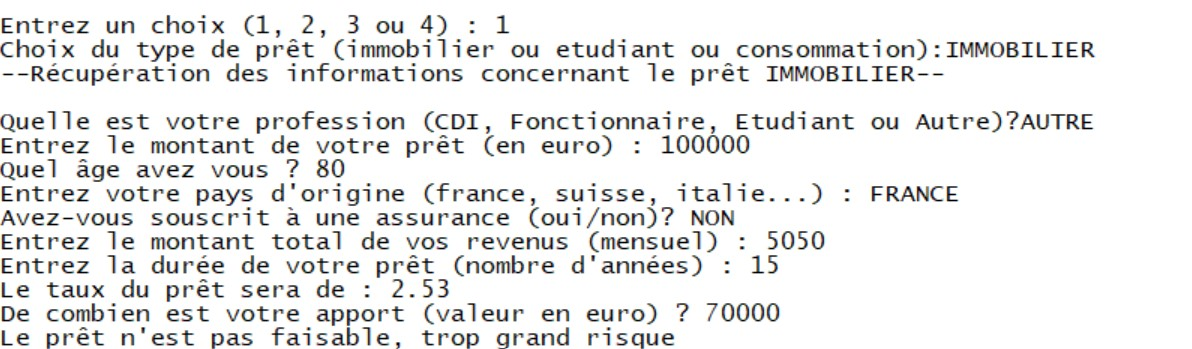
\includegraphics{img/fpret_impossible_age.jpg}
\caption{Faisabilitée d'un prêt immobilier impossible à cause de l'âge}
\end{figure}

\begin{figure}[H]
\centering
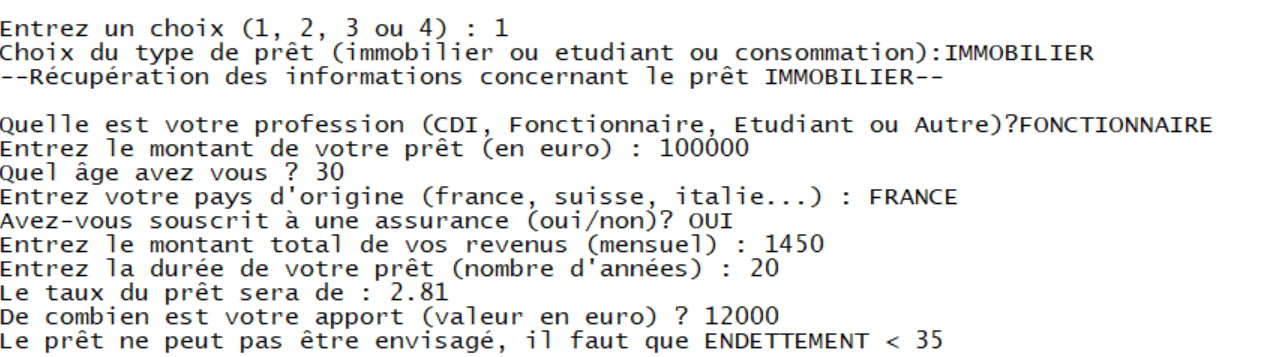
\includegraphics{img/fpret_impossible_endettement.jpg}
\caption{Faisabilitée d'un prêt immobilier impossible à cause de
l'endettement}
\end{figure}

La figure 4 montre un prêt impossible dû à l'âge. En effet,
l'utilisateur a entré un âge de 80 ans sans assurance. Or, par la règle
8, on remarque qu'il est impossible de contracter un prêt pour une
personne ayant plus de 65 ans et ne souscrivant pas à une assurance.\\
Dans la figure 5, on remarque que le prêt est refusé, car le taux
d'endettement est trop élevé. En effet, celui-ci ne doit pas dépasser 35
\%.

Enfin, la troisième fonctionnalité permet de calculer la durée d'un
prêt.

\begin{figure}[H]
  \centering
  
\includegraphics{img/calcul_duree_possible.jpg}
  \caption{Calcul mensualité possible}
\end{figure}

Dans cet exemple, l'utilisateur cherche à rembourser un prêt de 99 500€
avec une mensualité de 1 215€. Le moteur permet de définir la durée de
remboursement avec ces paramètres. Il nous renvoie qu'avec cette
mensualité, le prêt peut être remboursé en 7 ans.

\begin{figure}[H]
\centering
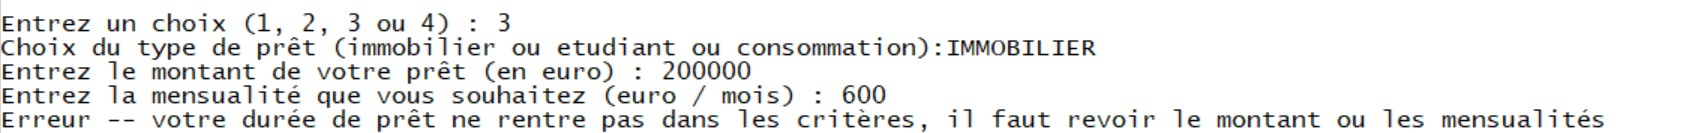
\includegraphics{img/calcul_duree_impossible.jpg}
\caption{Calcul mensualité impossible}
\end{figure}

Enfin, ce dernier exemple, renvoie une erreur, car il est impossible de
rembourser un prêt de 200 000€ avec des mensualités de 600€.

Ensuite, la seconde fonctionnalité permet de calculer les mensualités
d'un prêt. 

\begin{figure}[H]
  \centering
  
\includegraphics{img/calcul_montant_possible.jpg}
  \caption{Calcul durée possible}
\end{figure}

Dans cet exemple, l'utilisateur cherche à rembourser un prêt de 99 500€
en 26 ans. Le moteur permet de définir que cet utilisateur devra
rembourser environ 327.87€ par mois.

\begin{figure}[H]
  \centering
  
\includegraphics{img/calcul_montant_impossible.jpg}
  \caption{Calcul durée impossible}
\end{figure}


Dans ce second exemple, on remarque que le moteur ne calcule pas la mensualité demandée
par l'utilisateur. En effet, la durée du prêt n'est pas adéquate pour le
remboursement. Cette erreur peut être due à deux facteurs : le premier
est une durée de prêt trop longue et le second est une durée trop courte
pour permettre le remboursement. Dans notre cas, ce prêt est refusé, car
la durée du prêt est trop longue.

\pagebreak

\hypertarget{conclusion}{%
\section{Conclusion}\label{conclusion}}

Pour conclure, ce TP a été très instructif. Il nous a permis de mettre
en place un système-expert d'ordre 0+ de sa phase d'expertise à sa phase
d'utilisation.\\
Nous avons tout d'abord fait des recherches sur le domaine d'expertise
de notre système. Ensuite, nous avons formalisé la base de règles afin
que celle-ci soit utilisable par notre système et enfin nous avons
réalisé un ensemble de fonctions outils, de moteurs d'inférence ainsi
qu'une fonction principale afin de permettre le bon fonctionnement de
notre système.

Concernant la répartition des tâches, elles ont été réparties
équitablement tout au long de notre TP (comme dans les TPs précédents).
Une bonne dynamique de travail s'est installée, nous nous sommes tous les
deux investis dans les trois TPs.

\end{document}
